% Created 2026-06-19 Fri 05:09
% Intended LaTeX compiler: pdflatex
\documentclass[presentation]{beamer}
\usepackage[utf8]{inputenc}
\usepackage[T1]{fontenc}
\usepackage{graphicx}
\usepackage{longtable}
\usepackage{wrapfig}
\usepackage{rotating}
\usepackage[normalem]{ulem}
\usepackage{amsmath}
\usepackage{amssymb}
\usepackage{capt-of}
\usepackage{hyperref}
\usepackage[T1]{fontenc}
\usepackage[utf8]{inputenc}
\usepackage[spanish]{babel}
\usepackage[backend=biber, style=apa]{biblatex}
\addbibresource{/home/anthony-el/expo/BusesDelSistema_G1-G2/bibliography/bibliography.bib}
\author{G1 - G2}
\date{2026-06-18}
\title{S8 — Buses del Sistema}
\hypersetup{
 pdfauthor={G1 - G2},
 pdftitle={S8 — Buses del Sistema},
 pdfkeywords={},
 pdfsubject={},
 pdfcreator={Emacs 27.1 (Org mode 9.3)}, 
 pdflang={Spanish}}
\begin{document}

\maketitle
\tableofcontents


\section{Indicaciones}
\label{sec:org89cfee9}
\subsection{Indicaciones}
\label{sec:org3fa0817}
\begin{itemize}
\item Recuerde que si \texttt{options: H:2}, entonces:
\begin{itemize}
\item \texttt{*} Declara el nombre de la Sección
\item \texttt{**} Declara el nombre de la diapositiva
\end{itemize}
\item Puede alterar la estructura de la diapositiva si lo considera necesario
\item Reparto del tema por grupos:
\begin{itemize}
\item \textbf{G1:} Estructuras de Interconexión, Interconexión punto a punto, QPI
\item \textbf{G2:} Interconexión con Buses, Jerarquía de Buses, Elementos de Diseño, PCI Express
\end{itemize}
\item Para este tema consulte las siguientes fuentes:
\begin{itemize}
\item \textcite{stallings2006esp}, 7ma edición, 2006, Español, páginas 99 a 119.
\item \textcite{stallings2022computer}, 11ava edición, 2022, English, páginas 116 a 131.
\end{itemize}
\item Las tuplas (7, 99) significan: Edición 7, página 99 del PDF.
\item El grupo expone el tema y sube la presentación (\texttt{.ORG} y \texttt{.PDF} para Beamer, o \texttt{.ORG} y \texttt{.HTML} para reveal.js)
\item El grupo sube las ayudas memoria/notas del tema usando la plantilla \url{FormatoTareas/TemplateNotasClase.org} (\texttt{.ORG} y \texttt{.PDF})
\end{itemize}
\subsection{Diseño de las Diapositivas}
\label{sec:orgc9ae8cc}
\begin{itemize}
\item Para diseñar sus diapositivas puede consultar cualquiera de las
presentaciones \texttt{.ORG} desarrolladas por el profesor así como al
archivo \href{https://github.com/LeninGF/EPN-Lectures/blob/main/iccd332ArqComp-2024-B/Tutoriales/Beamer-Emacs/tutorialBeamer.org}{tutorialBeamer.org} en el repositorio de la clase.
\item Recuerde que los archivos \texttt{.ORG} son archivos de texto así que los
puede copiar y sustituir por su texto propio.
\end{itemize}
\subsection{Sobre este Documento}
\label{sec:orgd27a5c7}
\begin{itemize}
\item Este documento tiene la propuesta de temas a tratar y desarrollar
por los estudiantes.
\item Se ha de utilizar como base la bibliografía recomendada, pero puede
consultar bibliografía adicional.
\end{itemize}
\section{Buses del Sistema}
\label{sec:org6a69aef}
\subsection{Estructuras de Interconexión (7, 97)}
\label{sec:org54d0926}
\section{Interconexión con Buses}
\label{sec:org661e7b8}
\subsection{Interconexión con Buses (7, 99)}
\label{sec:org2177324}
\begin{itemize}
\item Un computador consta de tres componentes fundamentales: \textbf{CPU},
\textbf{Memoria} y \textbf{Módulos de E/S}.
\item Estos componentes deben comunicarse entre sí para ejecutar
programas.
\item La estructura de interconexión es el conjunto de caminos que
conectan estos módulos.
\item El diseño depende de los intercambios que deban realizarse:
\begin{itemize}
\item \textbf{Memoria a CPU}: La CPU lee una instrucción o dato desde la
memoria.
\item \textbf{CPU a Memoria}: La CPU escribe un dato en la memoria.
\item \textbf{E/S a CPU}: La CPU lee datos de un dispositivo de E/S mediante el
módulo correspondiente.
\item \textbf{CPU a E/S}: La CPU envía datos o comandos al dispositivo de E/S.
\item \textbf{E/S a/desde Memoria}: Utilizado en transferencias directas sin
pasar constantemente por la CPU (e.g., DMA - Acceso Directo a
Memoria).
\begin{center}
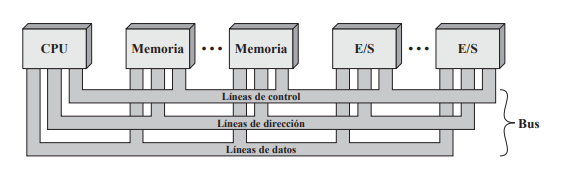
\includegraphics[width=.9\linewidth]{./images/ComponentesBus.png}
\end{center}
\end{itemize}
\end{itemize}

\subsection{Conceptos y Estructura Física}
\label{sec:org38f523d}
\begin{enumerate}
\item ¿Qué es un Bus?
\label{sec:org3b0387b}
\begin{itemize}
\item Un \textbf{bus} es un camino de comunicación compartido que conecta dos o
más dispositivos.
\item \textbf{Medio de difusión (broadcast)}: Las señales transmitidas por un
dispositivo son recibidas por todos los demás.
\item Si dos dispositivos transmiten al mismo tiempo, sus señales
colisionarán y se corromperán.
\item Por ende, solo \textbf{un dispositivo} puede transmitir datos con éxito en
un instante dado.
\item Los buses del sistema modernos constan de decenas de líneas de
comunicación individuales.
\end{itemize}
\end{enumerate}
\subsection{Estructura del Bus  (7, 99)}
\label{sec:org576dc1a}
Un bus de sistema se divide en tres grupos funcionales de líneas:

\begin{itemize}
\item \textbf{Bus de Datos}: 
\begin{itemize}
\item Proporciona un camino para transmitir datos entre los módulos.
\item El número de líneas determina el \textbf{ancho del bus de datos} (e.g.,
32, 64 o 128 bits).
\item El ancho del bus influye directamente en el rendimiento del
sistema.
\end{itemize}

\item \textbf{Bus de Direcciones}:
\begin{itemize}
\item Determina el origen o el destino del dato en el bus de datos.
\item Si la CPU desea leer una palabra de memoria, coloca la dirección
física de la palabra en estas líneas.
\item El \textbf{ancho del bus de direcciones} determina la capacidad máxima de
memoria direccionable del sistema (\(2^{n}\) ubicaciones).
\end{itemize}

\item \textbf{Bus de Control}:
\begin{itemize}
\item Controla el acceso y uso de las líneas de datos y direcciones.
\item Transmite órdenes y señales de temporización entre los módulos.
\item \textbf{Señales típicas}: Escritura/Lectura de Memoria, Escritura/Lectura
de E/S, Petición de Bus, Concesión de Bus, Reloj, Reinicio.
\begin{center}
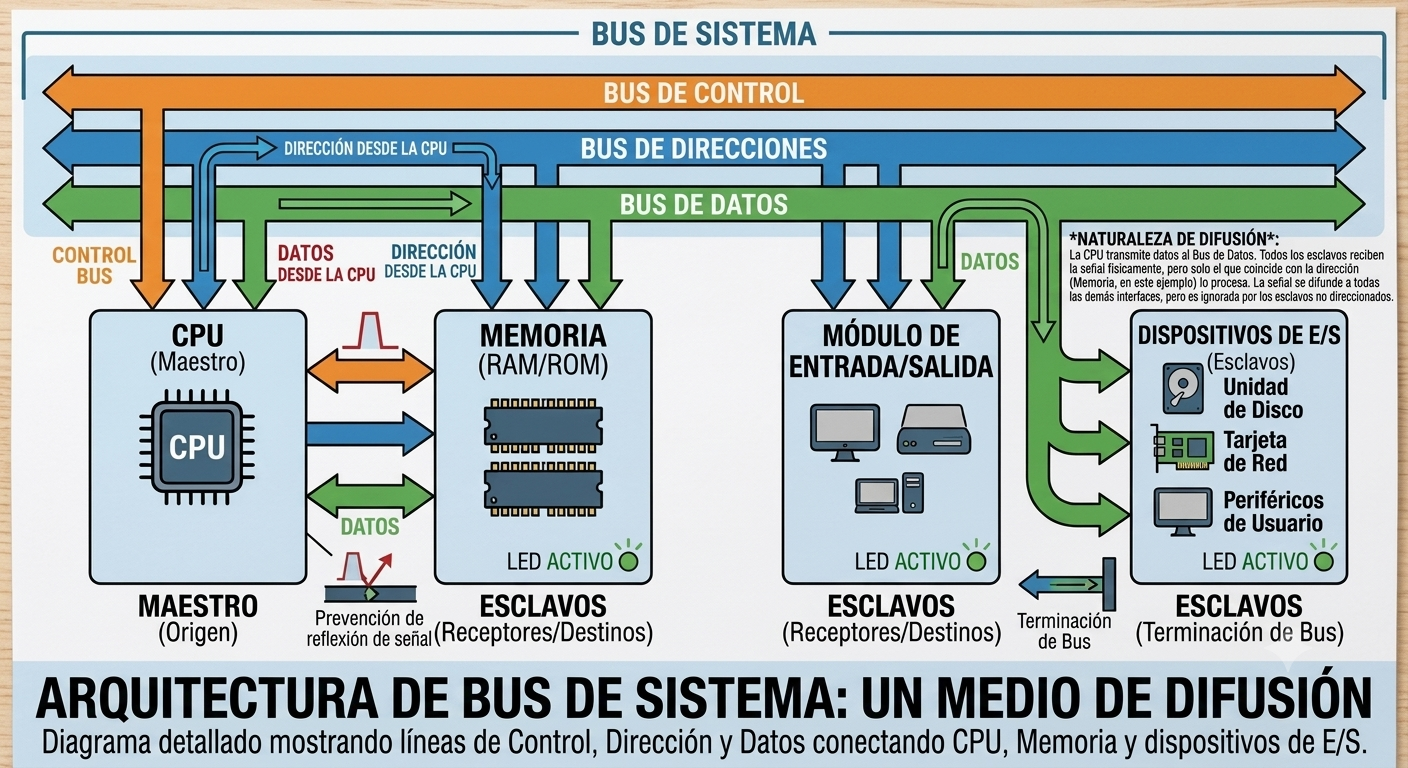
\includegraphics[width=.9\linewidth]{./images/TipoLineas.png}
\end{center}
\end{itemize}
\end{itemize}

\subsection{¿Por qué surge la Jerarquía de Buses? (7, 102)}
\label{sec:org640aee0}
-\textbf{¿Por qué surge la jerarquía de buses?}
\begin{itemize}
\item Un único bus compartido simplifica la interconexión del sistema.
\item A medida que aumenta el número de dispositivos, aparecen limitaciones críticas:
\begin{itemize}
\item \textbf{Retardo de propagación:} Las líneas físicas largas ralentizan las señales.
\item \textbf{Contención:} Más dispositivos compiten por el acceso al canal.
\item \textbf{Tráfico masivo:} El flujo de datos entre CPU, memoria y E/S satura el canal.
\end{itemize}
\item \textbf{Resultado:} El bus se convierte en un \textbf{\textbf{cuello de botella}} y un único bus ya no puede satisfacer a todos los componentes.
\end{itemize}

\subsection{Jerarquía Tradicional de Buses (7, 102)}
\label{sec:org2ac5dc1}
\begin{enumerate}
\item Arquitectura Clásica
\label{sec:org692174f}
\begin{center}
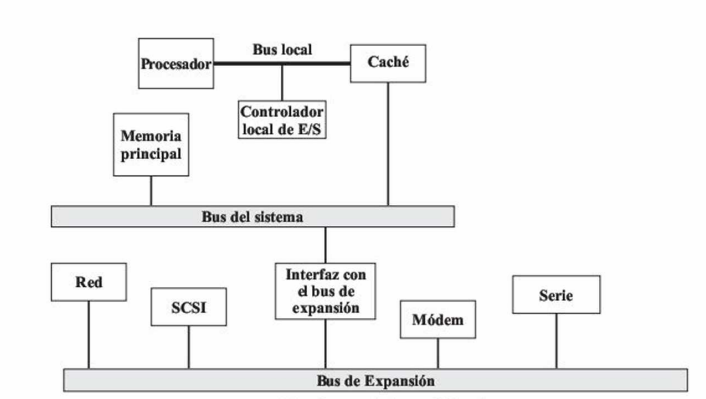
\includegraphics[width=\textwidth]{./images/JerarquiaTradicionalBus.png}
\end{center}

\item Características
\label{sec:orgbc0b48a}
\begin{itemize}
\item \textbf{Bus Local:} Conecta la CPU con la memoria caché a la máxima velocidad del procesador.
\item \textbf{Bus del Sistema:} Se encarga de conectar la caché con la memoria principal.
\item \textbf{Bus de Expansión:} Conecta los dispositivos de E/S periféricos.
\item \textbf{Aislamiento:} Mantiene el tráfico de E/S separado de los procesos de la CPU.
\end{itemize}
\end{enumerate}

\subsection{Jerarquía de Buses de Altas Prestaciones (7, 103)}
\label{sec:orga8b6cfa}

\begin{enumerate}
\item Arquitectura Moderna
\label{sec:org904ef67}
\begin{center}
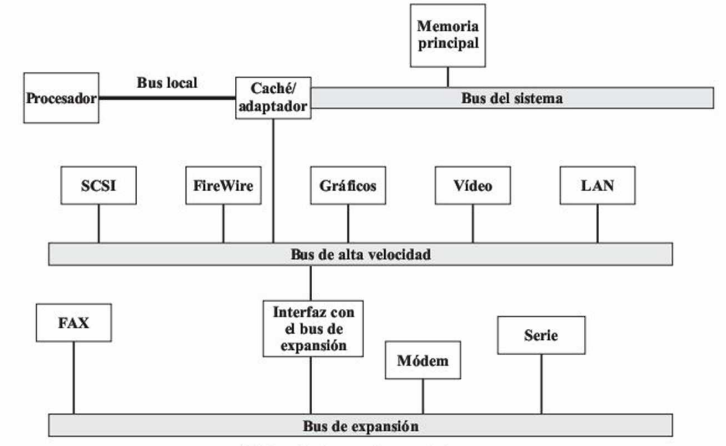
\includegraphics[width=\textwidth]{./images/JerarquiaAltasPrestaciones.png}
\end{center}

\item Características
\label{sec:org38844ac}
\begin{itemize}
\item \textbf{Bus de Alta Velocidad:} Conecta de forma más directa los dispositivos exigentes (video, gráficos, redes rápidas).
\item \textbf{Bus de Expansión:} Mantiene relegados a los dispositivos y periféricos más lentos.
\item \textbf{Ventaja:} La separación del tráfico mejora el rendimiento global del sistema.
\item \textbf{Transición:} Esta organización introduce nuevos retos en el arbitraje, la temporización y el ancho del bus.
\end{itemize}
\end{enumerate}

\subsection{Elementos de Diseño de un Bus (7, 104)}
\label{sec:orgc919ff3}
\begin{itemize}
\item El diseño de un bus de sistema no es arbitrario; representa un balance
crítico entre \textbf{costo físico}, \textbf{complejidad del hardware} y
\textbf{rendimiento esperado}.
\item Para evaluar o diseñar un bus, Stallings define los siguientes parámetros clave:
\begin{itemize}
\item \textbf{Físicos}: Tipo de líneas y ancho del bus.
\item \textbf{Lógicos y de Control}: Método de arbitraje, tipo de transferencia y temporización.
\end{itemize}
\item A continuación, se analizará cómo cada uno de estos elementos impacta directamente en el ancho de banda del procesador y el direccionamiento del sistema.
\end{itemize}

\section{Tipos de Líneas de Bus}
\label{sec:orgcd7b88c}

\section{Tipos de Líneas de Bus}
\label{sec:org815a2b8}
\subsection{Clasificación por Funcionalidad}
\label{sec:orgcfcde03}
\begin{enumerate}
\item Líneas Dedicadas vs Multiplexadas
\label{sec:orgffe3f9b}
\begin{itemize}
\item \textbf{Dedicadas}:
\begin{itemize}
\item Asignadas permanentemente a una función o subconjunto de
componentes.
\item Ejemplo: Líneas de direcciones y de datos físicamente separadas.
\item +Rendimiento alto, -Costo de espacio y pines.
\end{itemize}
\item \textbf{Multiplexación Temporal}:
\begin{itemize}
\item El mismo conjunto de líneas se usa para diferentes propósitos en
tiempos distintos.
\item Ejemplo: Las mismas líneas envían la dirección al inicio y luego
el dato.
\item +Ahorro de espacio y pines, -Lógica de control compleja y
velocidad.
\end{itemize}
\end{itemize}
\end{enumerate}
\section{Arbitraje del Bus}
\label{sec:orgd289b9f}
\subsection{Métodos de Control}
\label{sec:orgdbcdf7d}
\begin{enumerate}
\item Arbitraje Centralizado vs Distribuido
\label{sec:org28c27f7}
\begin{enumerate}
\item Centralizado\hfill{}\textsc{Texto:BMCOL}
\label{sec:orga4aebaa}
\begin{itemize}
\item Un solo hardware (\textbf{árbitro}) asigna el acceso.
\item Proceso: Petición \(\rightarrow\) Concesión.
\item Punto único de fallo.
\end{itemize}
\item Distribuido\hfill{}\textsc{Imagen:BMCOL}
\label{sec:org2473585}
\begin{itemize}
\item No hay nodo central.
\item Cada módulo tiene lógica propia.
\item Cooperación mediante protocolos compartidos.
\end{itemize}
\end{enumerate}
\end{enumerate}

\section{Temporización}
\label{sec:org170155f}
\subsection{Coordinación de Eventos}
\label{sec:org0f9117f}
\begin{enumerate}
\item Temporización Síncrona
\label{sec:org6dff327}
\begin{itemize}
\item Determinada por una señal de \textbf{reloj del sistema}.
\item Todos los dispositivos ven el tren de pulsos (0 y 1).
\item Las acciones ocurren en ciclos de reloj fijos.
\item \textbf{Ventaja}: Simple y rápida de probar.
\item \textbf{Desventaja}: El dispositivo más lento limita al bus entero.
\end{itemize}

\item Temporización Asíncrona
\label{sec:org1b08da1}
\begin{itemize}
\item La ocurrencia de un evento depende del éxito del evento anterior.
\item Utiliza un protocolo de saludo (\textbf{handshaking}).
\item \([REQ] \rightarrow [ACK] \rightarrow [Data]\)
\item \textbf{Ventaja}: Mezcla eficiente de dispositivos rápidos y lentos.
\item \textbf{Desventaja}: Implementación de hardware muy compleja.
\end{itemize}
\end{enumerate}

\section{Ancho de Bus y Transferencia}
\label{sec:org89d89fd}
\subsection{Parámetros de Rendimiento}
\label{sec:orge8bcd0f}
\begin{enumerate}
\item Ancho del Bus
\label{sec:org6b68084}
\begin{enumerate}
\item Datos\hfill{}\textsc{BMCOL}
\label{sec:org77aed46}
\begin{itemize}
\item Determina cuántos bits se transmiten en paralelo.
\item A mayor ancho, mayor rendimiento del sistema.
\end{itemize}
\item Direcciones\hfill{}\textsc{BMCOL}
\label{sec:org18845a1}
\begin{itemize}
\item Determina el rango de memoria direccionable.
\item Capacidad máxima: \(2^{n}\) bytes.
\end{itemize}
\end{enumerate}

\item Tipos de Transferencia de Datos
\label{sec:orgf1ae6b9}
\begin{itemize}
\item \textbf{Lectura/Escritura}: Operación básica de memoria.
\item \textbf{Lectura-Modificación-Escritura}: 
\begin{itemize}
\item Operación atómica indivisible.
\item Clave para sincronización y semáforos.
\end{itemize}
\item \textbf{Transferencia por Bloques}:
\begin{itemize}
\item Envía 1 dirección y luego una ráfaga de datos.
\item Optimiza el uso de la memoria Caché y DMA.
\end{itemize}
\end{itemize}
\end{enumerate}

\section{Interconexión punto a punto}
\label{sec:orgcb8bd89}
\subsection{Problemas del bus compartido tradicional}
\label{sec:org4127a43}
\begin{center}
\includegraphics[width=.9\linewidth]{./images/BusCuelloDeBotella.jpeg}
\end{center}
-Restricciones eléctricas: Al subir la frecuencia del reloj para ganar velocidad, el bus tradicional falla\\[0pt]
-El problema: Con tasas de datos tan altas, es casi imposible realizar la sincronización y el arbitraje a tiempo y sin errores\\[0pt]
\subsection{El Reemplazo: Interconexión Punto a Punto}
\label{sec:orgf7640c7}
\begin{center}
\includegraphics[width=.9\linewidth]{./images/InterconexionPuntoaPunto.jpeg}
\end{center}
-El nuevo estándar: El bus compartido ha sido reemplazado casi por completo por interconexiones punto a punto\\[0pt]
-Ventajas: Menos latencia, una tasa de datos significativamente más alta y mejor escalabilidad\\[0pt]
\subsection{El Reemplazo: Las 3 características modernas}
\label{sec:org70c82b3}
\begin{center}
\includegraphics[width=.9\linewidth]{./images/CapasIPP.jpeg}
\end{center}
\begin{enumerate}
\item Conexiones directas por parejas: Al enlazar directamente dos componentes, se elimina por completo la necesidad de arbitraje
\item Arquitectura de protocolos en capas: Se estructuran de forma similar a las redes de datos (como TCP/IP)
\item Transferencia por paquetes: Los datos se envían como secuencias de paquetes que incluyen cabeceras y detección de errores
\end{enumerate}
\subsection{QPI (11, 120): Ejemplo de Interconexión Punto a Punto: Intel QPI?}
\label{sec:org2d3b53f}
\begin{itemize}
\item \textbf{\textbf{Interconexión punto a punto}} de alta velocidad introducida en 2008 \autocite[p.118]{stallings2022computer}.
\item \textbf{\textbf{Motivación:}} Superar restricciones eléctricas y latencia de los
buses compartidos en chips multinúcleo.
\item \textbf{\textbf{Pilares:}}
\begin{itemize}
\item Conexiones directas por pares (sin arbitraje).
\item Arquitectura de protocolo en capas.
\item Transferencia de datos mediante paquetes con control de errores.
\end{itemize}
\end{itemize}

\subsection{Configuración Multinúcleo y Red de Conmutación}
\label{sec:org4c7903f}
\begin{enumerate}
\item Imagen QPI\hfill{}\textsc{Imagen}
\label{sec:orgcfc1d77}
\begin{center}
\includegraphics[width=0.9\textwidth]{./images/MulticoreConfigurationQPI.png}
\end{center}

\item Explicación\hfill{}\textsc{Texto}
\label{sec:org1775041}
\begin{itemize}
\item Los enlaces QPI (flechas verdes) forman una \textbf{malla de conmutación} (switching fabric).
\item Permite que los datos "salten" entre núcleos para llegar a su destino.
\item Conecta el procesador con el I/O Hub (IOH), que traduce señales hacia dispositivos PCIe.
** Configuración Multinúcleo y Red de Conmutación
\end{itemize}
\end{enumerate}

\subsection{Arquitectura de 4 Capas de QPI}
\label{sec:org316f4af}
\begin{center}
\includegraphics[width=0.5\textwidth]{./images/QPILayers.png}
\end{center}

\begin{itemize}
\item \textbf{\textbf{Protocolo:}} Reglas de alto nivel y coherencia de caché.
\item \textbf{\textbf{Encaminamiento (Routing):}} Tablas de ruta definidas por firmware.
\item \textbf{\textbf{Enlace (Link):}} Transmisión confiable y control de flujo por Flits.
\item \textbf{\textbf{Física:}} Unidades eléctricas y lógica de bits (Phits).
\end{itemize}

\subsection{Capa Física: Phits y Señalización Diferencial}
\label{sec:orga1c8e29}

\begin{center}
\includegraphics[width=0.45\textwidth]{./images/PhysicalInterfaceQPIInterconnect.png}
\end{center}

\begin{itemize}
\item \textbf{\textbf{Phit (Physical Unit):}} Unidad mínima de 20 bits.
\item \textbf{\textbf{Señalización Diferencial (LVDS):}} Compara voltajes entre dos cables para reducir ruido.
\item \textbf{\textbf{Capacidad:}} Hasta 6.4 GT/s (transferencias por segundo), moviendo
hasta 32 GB/s.
\end{itemize}

\subsection{Capa Física: Distribución Multicarril}
\label{sec:org28bab5e}

\begin{enumerate}
\item Imagen\hfill{}\textsc{Imagen}
\label{sec:orgb95be31}
\begin{center}
\includegraphics[width=0.9\textwidth]{./images/DistribucionMulticarrilQPI.png}
\end{center}

\item Explicación\hfill{}\textsc{Texto}
\label{sec:orgd62fc84}
\begin{itemize}
\item El puerto QPI usa 20 carriles (\textbf{lanes}) de datos en cada dirección.
\item Los bits de un Flit se reparten entre los carriles usando técnica \textbf{round‑robin}.
\item Permite la transmisión de un Phit completo (20 bits) en paralelo por ciclo.
\end{itemize}
\end{enumerate}

\subsection{Capa de Enlace: Flits y Control de Flujo}
\label{sec:orgb4cfad1}
\begin{itemize}
\item \textbf{\textbf{Flit (Flow Control Unit):}} PDU de 80 bits (72 de mensaje + 8 de CRC).
\item \textbf{\textbf{Control de errores:}} Si el CRC falla, el receptor solicita retransmisión inmediata.
\item \textbf{\textbf{Esquema de Créditos:}} El receptor devuelve créditos al emisor cuando su buffer tiene espacio, evitando saturación.
\end{itemize}

\subsection{Capas de Encaminamiento y Protocolo}
\label{sec:orgfefc71e}
\begin{itemize}
\item \textbf{\textbf{Encaminamiento:}} Decide el camino del paquete a través de los nodos del sistema usando tablas de rutas.
\item \textbf{\textbf{Protocolo:}} Maneja la coherencia de caché, asegurando que todos los núcleos vean el dato más actualizado de la memoria.
\item \textbf{\textbf{Unidad de mensaje:}} El "Paquete", que consiste en un número entero de Flits.
\end{itemize}

\section{PCI Express}
\label{sec:org3368e70}
\subsection{PCI Express (11, 123)}
\label{sec:org47fa332}
\section{Referencias}
\label{sec:org73c4a49}
\subsection{Bibliografía}
\label{sec:orge8b6685}
\printbibliography
\end{document}
